\documentclass[a4paper]{IEEEtran}
\usepackage[utf8]{inputenc}
\usepackage[T1]{fontenc}
\usepackage{amsfonts, amsthm,amsmath}
\usepackage{graphicx}

\title{Civilizacije}
\author{Anže Marinko, Klara Golob, Ema Jemec in mentor dr. Matjaž Gams \\ Inštitut Jožef Stefan (E9 - oddelek za inteligentne sisteme), Ljubljana \\ Samo za interno uporabo \\ maj 2020}

\begin{document}

\maketitle
\tableofcontents

\section{Uvod}

Oceniti želimo porazdelitev časa, ki ga inteligentna civilizacija preživi v naši galaksiji (in posplošeno v celotnem vesolju). Civilizacija se šteje za inteligentno, če je sposobna radio-komunikacije z drugimi planeti. Porazdelitev ocenjujemo z uporabo Drakeove enačbe. Želimo pa zajeti čim večji prostor relevantnih modelov. Relevantni modeli so tiste porazdelitve, ki ne dajejo prevelike verjetnosti temu, da bi inteligentna civilizacija obstajala več milijonov let in ki imajo s časom padajočo gostoto, torej da je bolj verjetno, da bi obstajali (bili sposobni radio-komunikacije) le tisoč let kakor pa med tisoč in dvatisoč let.

Pripravili smo tri bolj splošne modele, katerim smo spreminjali parametre, da bi dobili čim več različnih porazdelitev, ki ustrezajo Drakeovi enačbi. Vse te porazdelitve smo potem gručili po podobnosti in dobili nekaj značilnih porazdelitev, ki jih lahko posamično obravnavamo in izključujemo z razvojem znanosti in vedenja o vesolju. To nam pomaga oceniti, koliko let obstoja še preostaja naši civilizaciji na tem planetu. Če je verjetnost, da obstajamo še dolgo, majhna, se moramo toliko bolj potruditi, da ne propademo že prej.

Vsa koda je pripravljena v programskem jeziku Python 3, kakih 470 vrstic urejene kode s komentarji.

\section{Osnovni modeli in njihova posplošitev}

V nadaljevanju vam bomo predstavili razširjen Sandbergov model in dva druga modela dobljena s spremembo prvega. Vsak model pa je odvisen od nekaj parametrov, za katere znamo ceniti spodnjo in zgornjo mejo, ne vemo pa njihove dejanske vrednosti ali celo porazdelitve na tem intervalu. Za razliko od Sandberga bomo namesto fiksnih vrednosti uporabili različne porazdelitve na izbranem intervalu. Vsak parameter porazdelimo z eno izmed petih izbranih porazdelitev ter tako dobimo možnih izbranih porazdelitev $5^{\#parametrov}$ za vsako zgornjo mejo za $N$ za vsak model.

Izbrane porazdelitve so:
\begin{enumerate}
	\item loguniformna (uniformno porazdeljeno glede na x os v logaritmski skali),
	\item uniformna (enakomerno po celem intervalu),
	\item pol Gaussova (polovica Gaussove porazdelitve z vrhom pri spodnji meji),
	\item lognormal (normalna porazdelitev vzdolž x osi v logaritmski skali s povprečjem na sredini intervala),
	\item fiksna (fiksirana vrednost na zgornji meji).
\end{enumerate}

Poleg tega ne poznamo zgornje meje za število inteligentnih civilizacij v nekem trenutku $N$. Edino, kar vemo, je, da obstaja vsaj ena civilizacija (to smo mi) in domnevamo, da inteligentnih civilizacij v naši galaksiji ni več kot 10 000, sicer bi kakšne druge civilizacije že videli ali vsaj zaznali njihove radijske valove, kar bi šteli za inteligentno civilizacijo.

\subsection{Model 1}

Imamo 6 parametrov:
\begin{enumerate}
	\item $R_\ast$ stopnja nastanka nove zvezde, kar je porazdeljeno nekje med 1 in 100 na leto
	\item $f_p$ verjetnost, da ima zvezda vsaj en planet, je porazdeljena med 10 in 100 odstotki
	\item $f_e$ verjetnost, da je ta planet podoben zemlji, je nekje med 10 in 100 odstotki
	\item $f_i$ verjetnost, da se na zemlji podobnem planetu razvijejo inteligentna bitja, je porazdeljena med 0,1 in 100 odstotki
	\item $f_c$ verjetnost, da ta bitja naredijo civilizacijo sposobno radio-komunikacje z drugimi planeti, je med enim in 100 odstotki
	\item $N$ - število takih civilizacij v naši galaksiji porazdeljena med 1 in izbrano zgornjo mejo za število civilizacij
\end{enumerate}

Število let obstoja civilizacije $L$ je po Drakeovi enačbi enako $L = N / (R_\ast f_p f_e f_i f_c)$. Ker so vsi parametri slučajne spremenljivke je tudi $L$ slučajna spremenljivka, katere porazdelitev empirično dobimo z veliko generiranimi primeri.

Tako dobimo za izbrane porazdelitve in zgornjo mejo za $N$ možno porazdelitev, torej $5^6$ različnih porazdelitev za vsako izbrano zgornjo mejo za $N$. Enako velja tudi za preostale modele.

\subsection{Model 2}

V drugem modelu zberemo nekatere parametre iz prvega modela skupaj tako, da imamo le tri parametre. Za razliko od prvega modela, ki po Drakeovi enačbi računa glede na število inteligentnih civilizacij v tem trenutku, drugi model uporablja namesto stopnje nastanka nove zvezde kar število vseh zvezd. Parametre pa združi zgolj v tri:
\begin{enumerate}
	\item astro-fizična verjetnost $f_a$ porazdeljena lognormalno na sredini intervala od  ob robovih pa z izbrano porazdelitvijo
	\item bio-tehnična verjetnost $f_b$ porazdeljena med $10^{-11}$ in 0.1 odstotka,
	\item $N$ - število takih civilizacij v naši galaksiji porazdeljena med 1 in izbrano zgornjo mejo za število civilizacij.
\end{enumerate}

Tu je $L$ ponovno izračunan kot $N / (f_a + f_b)$.

\subsection{Model 3}

Modelu 1 dodamo možnost širjenja na druge planete. Izračunamo parametre za model 1:
$N$ in $f := R_\ast f_p f_e f_i f_c$, kjer je $f$ stopnja nastanka nove inteligentne civilizacije.

$E = 5.1334 * 10^{10 + f_p + f_e} S$ je ocenjeno število zemlji podobnih planetov, kjer je $S = 4.7233 * 10^{-42}$ gostota zvezd glede na Wikipedijo.

Iščemo ničle polinoma $p(L) = E f L^4 + f L - N$ oz. rešitev enačbe $f * (L + E L^4) = N$, kjer je $L$ pozitivna realna ničla polinoma oz. pozitivna realna rešitev enačbe.

\subsection{Implementacija}

Za pripravo vsakega histograma za vsako kombinacijo porazdelitev in zgornje meje za $N$ smo generirali 200 000 točk in jih združili v histograme z intervalom razrezanim na 100 delčkov. Izračunali smo histogram, kjer smo imeli linearno in logaritmsko skalo na osi $L$.

Izračunali histograme za vse možne kombinacije porazdeltev
pri zgornjih mejah za število inteligentnih civilizacij $N$ nastavljenih na 1, 3, 10, 30, 100, 300, 1000, 3000 in 10 000.

Histogram smo naredili na intervalu $\lbrack 0, 10^10\rbrack$ pri linearni skali in $\lbrack -1, 12\rbrack$ pri logaritmski skali, ker večje vrednosti niso realne in so le teoretične dobljene zaradi posplošitev v modelu.

Pri generiranju podatkov smo izkosristili lastnost, da model 1 izračunamo tekom generiranja modela 3. Problem dopušča popolno paralelizacijo računanja vsakega histograma na svojem procesorju. V našem primeru smo uporabili 10 procesorskih enot. Histograme smo si tekom izračunavanja zapisovali v datoteke in jih na koncu združili v 4 datoteke. Posebej linearne in logaritmske histograme in za vsake histograme še sezname parametrov v drugi datoteki.

\section{Gručenje}

Vse dobljene histograme želimo posplošiti na le nekaj značilnih histogramov, ki nam povedo nekaj možnih porazdelitev vrednih razprave. Če želimo tudi vizualno prikazati množico histogramov, kjer bodo gruče kar se da opazne, moramo izrisati le tri dimenzije izmed vseh 100 (dolžina histograma). V nadaljevanju vam bomo predstavili transformacijo prostora tako, da bo slika kar se da povedna. Torej iščemo novo bazo za prostor histogramov.

\subsection{PCA - Principal component analysis}

Izračunamo korelacijsko matriko za vse histograme (dobimo $100\times100$ matriko) in izračunamo lasne vrednosti ter lastne vektorje korelacijske matrike. Vse histograme zamaknemo za povprečen histogram in jih preslikamo z matriko iz lastnih vektorjev.

Novo dobljene točke so v lastnem prostoru in če so lastne vrednosti urejene padajoče, so prve dimenzije najbolj informativne, ker nosijo največ variance. Velikost lastne vrednosti v primerjavi z vsoto lastnih vrednosti nam pove, koliko variance v podatkih nam ta dimenzija prinese. Torej vzamemo le največje tri lastne vrednosti za izris. Lastni vektorji pa so baza prostora. Inverzna transformacija je enostavna.

PCA ne vpliva na podobnost med histogrami (razdalje se pri rotaciji in translaciji ohranjajo).

\subsection{Analiza gruč}

Z uporabo algoritma k-means, ki točke iterativno gruči na podlagi k povprečij gruč, histograme razvrstimo v izbrano število gruč (smiselno je do 10). Vsako gručo analiziramo v smislu porazdelitve osnovnih modelov in izbranih zgornjih mej za $N$. Porazdelitve izpišemo na sledeč način:

Na primer za neko gručo:
\begin{center}
	\begin{tabular}{ l|ccc } 
	Model & 1 & 2 & 3 \\ \hline
	 & 523 & 425 & 3
	\end{tabular}
\begin{tabular}{ l|ccccccccc } 
	$N_{max}$ & 0 &	0.5&1 &1.5 &2 &2.5 &3 &	3.5&4 \\ \hline
	&25 &45 &60 &81&110 &148 &177 &165 &140
\end{tabular}
\end{center}

Poleg tega za vsako gručo izračunamo povprečno porazdelitev $f_i$ (in uporabimo inverzno transformacijo za izris), njeno preživetveno funkcijo ($G(t) = 1 - \int_0^t f_i(s) ds$) in konveksno ovojnico gruče, da lahko izberemo še nekaj robnih primerov iz gruče.

Ob izrisu prvih treh dimenzij transformiranega prostora histogramov s PCA točke obarvamo glede na osnovni model in velikost pike določimo kot $log(N_{max})$. Na sliko ne izrišemo vseh točk, da se lepše vidi in ker ima model 2 občutno manj primerov jih pa vse uporabimo pri računanju PCA, gruč in aproksimacije točk v 3-dimenzionalnem prostoru s ploskvijo. Aproksimiramo z linearno regresijo na podlagi prvih dveh dimenzij na tretjo dimenzijo. Implementirano imamo do ploskev stopnje 3, torej za izbrano gručo izračunamo koeficiente $b$ za ploskev: \begin{eqnarray}
x_3 &=& b_0 + b_1 x_1 + b_2 x_2 + b_3 x_1 x_2 + b_4 x_1^2 + b_5 x_2^2 + \nonumber \\
&+& b_6 x_1^2 x_2 + b_7 x_1 x_2^2 + b_8 x_1^3 + b_9 x_2^3. \nonumber
\end{eqnarray}
Izračunano ploskev tudi narišemo na 3-dimenzionalno sliko, kjer so točke in ploskve obarvane po gručah.












\section{Rezultati}

opažanja in predvidevanja ob slikah
\begin{figure}[h]
	\centering
	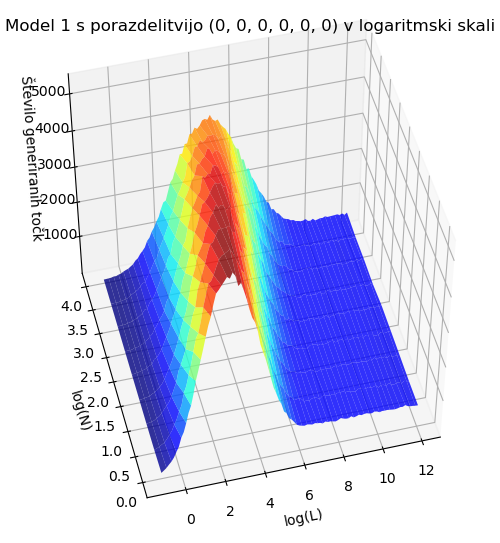
\includegraphics[width=0.9\linewidth]{Figures/porazdelitev3D}
	\caption{Histogrami za prvi model, kjer so vsi parametri porazdeljeni loguniformno.}
	\label{fig:porazdelitev3d}
\end{figure}

\begin{figure*}
	\centering
	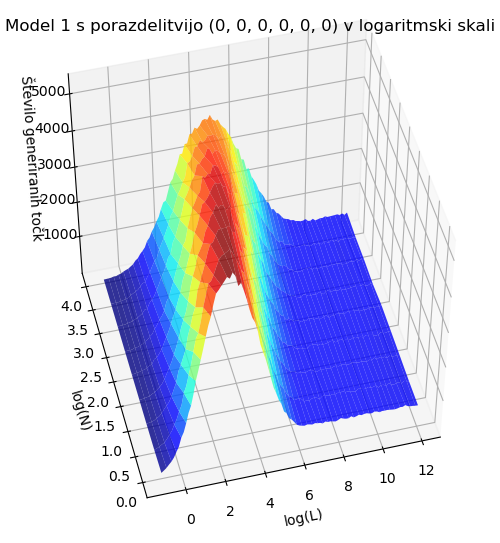
\includegraphics[width=0.7\linewidth]{Figures/porazdelitev3D}
	\caption{Histogrami za prvi model, kjer so vsi parametri porazdeljeni loguniformno.}
	\label{fig:porazdelitev3d}
\end{figure*}











\section{Razprava}

Želimo zapolniti še luknje v tem oblaku točk, da bi dobili čim bolj celostno podobo možnih histogramov. V nadaljevanju bomo dodali še četrti model, ki je povprečje modela 1 in 3 pri istih porazdelitvah in isti zgornji meji za $N$ ter eno izmed izmed porazdelitev iz modela 2 upoštevajoč porazdelitev iz prvih dveh modelov.

Peti model bi bil za vsako porazdelitev iz modela 2 povprečje z vsemi histogrami iz modela 1 in 3 s primerljivimi porazdelitvami. Prvih pet modelov bi nam tako že dali okrog 1 120 000 histogramov. Če pa kakšen izmed novih dveh modelov ne prinaša dovolj nove informacije oz. le zgosti porazdelitev točk v že gostih delih oblaka točk, se ga znebimo, ker želimo točke čim bolj enakomerno porazdeliti.

Poleg tega je že v pripravi nov model, ki veliko bolj pesimistično ocenjuje vrednosti parametrov in pravi, da je razvoj tovrstne civilizacije praktično nemogoč, torej da smo skoraj gotovo edini v vesolju. Ker pa ne vemo, kaj bi bilo realistično, ne vemo ali to tudi zares je preveč pesimistično. Ta teorija se imenuje Rare Earth theory.

Ko bomo imeli vse te modele pripravljene, bomo izračunali histograme na podlagi vsaj 5 milijonov generiranih točk za bolj gladke histograme in na večji množici zgornjih mej za $N$.

\end{document}
